\section{Methods}
This section outlines an alternative methodology for identifying moving flock patterns in large spatio-temporal datasets, utilizing modern distributed frameworks to partition and parallelize the workload.  Before discussing the details of our contributions, we will provide an overview of the current state-of-the-art to highlight the challenges and limitations in handling large spatio-temporal datasets.

\subsection{The BFE sequential algorithm}
The alternative approach we will discuss closely follows the steps outlined in \cite{vieira_2009}. In that work, the authors introduced the Basic Flock Evaluation (BFE) algorithm, designed to identify flock patterns in trajectory databases. While the full details of the algorithm can be found in the source, we will provide a general overview of the key aspects. It is important to note that the BFE algorithm operates in two phases: first, it identifies maximal disks at the current time step; second, it extends and reports previous flocks by combining them with the newly discovered disks.

The input for the BFE algorithm consists of a set of points, a minimum distance $\varepsilon$ (which defines the diameter of the disks where the moving entities must lie), a minimum number of entities $\mu$ per disk, and a minimum duration $\delta$, representing the required time units that entities must remain together to be considered a flock. Based on this input, Figure \ref{fig
} illustrates the workflow of the process in four general steps. The primary goal of this phase is to identify a set of disks at each time step, enabling the combination with future disks to form flocks.

\begin{figure}
    \centering
    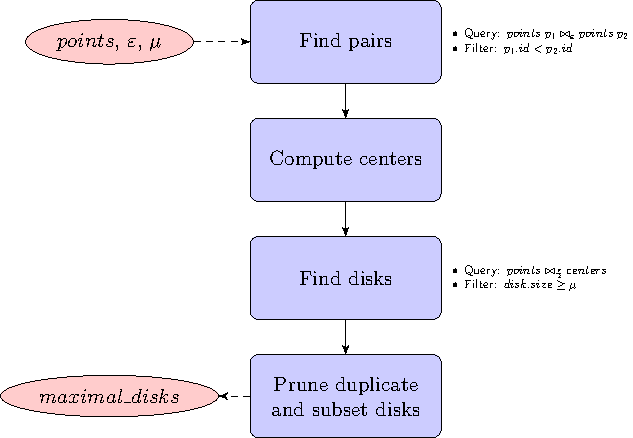
\includegraphics[width=\linewidth]{figures/MF_flowchart}
    \caption{General steps in phase 1 of the sequential algorithm.}\label{fig:MF_flowchart}
\end{figure}

The main steps in phase 1 follow:
\begin{enumerate}
    \item Pair finding:  The algorithm uses the parameter $\varepsilon$ to identify pairs of points that are within a maximum distance of $\varepsilon$ units from each other. This is achieved through a distance self-join operation on the set of points, using $\varepsilon$ as the distance threshold. To avoid redundancy, duplicate pairs are eliminated; for example, the pair $(p_1, p_2)$ is considered identical to the pair $(p_2, p_1)$, so only one instance is retained. Point IDs are used to filter out these duplicates efficiently.
    \item Center computation:  From the set of pairs obtained, each pair is used to compute the centers of two circles, each with a radius of $\frac{\varepsilon}{2}$, whose circumferences pass through the two points in the pair. The pseudo-code for this procedure is provided in Appendix \ref{app}.
    \item Disk finding: Once the centers have been identified, a query is executed to gather the points within a distance of $\varepsilon$ units from each center. This is accomplished by performing a distance join between the set of points and the set of centers, using $\frac{\varepsilon}{2}$ as the distance parameter. As a result, each disk is defined by its center and the IDs of the surrounding points. At this stage, a filter is applied to discard any disks that contain fewer than $\mu$ entities.
    \item Disk pruning: It is possible for a disk to contain the same set, or a subset, of points as another disk. In such cases, the algorithm reports only that one disk which contains the other(s), referred to as the \textit{maximal} disk. The procedure for identifying maximal disks is explained in Appendix \ref{app}.
\end{enumerate}

It is important to note that BFE also employs a grid structure in this phase to optimize spatial operations. The algorithm divides the space into a grid, where each cell has a side length of $\varepsilon$ (see Figure \ref{fig:grid} from \cite{vieira_2009}). This structure allows BFE to limit its processing to each grid cell and its eight neighboring cells. There is no need to query cells beyond this neighborhood, as points in more distant cells are too far away to influence the results.

\begin{figure}
    \centering
    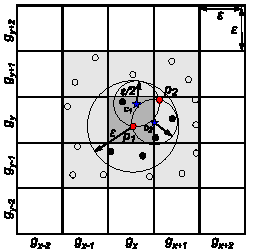
\includegraphics[width=0.6\linewidth]{figures/grid2}
    \caption{The grid-based structure proposed at \cite{vieira_2009}.}\label{fig:grid}
\end{figure}

Figure \ref{fig:FF_flowchart} explains schematically phase 2. This phase performs a recursion using the set of disks found at time $i$ and the set of partial flocks computed at the  previous time instant $i-1$.  As we do not know where and how far a group of points can move in the next time instant, this step performs a (temporal) join between both sets (partial flocks computed at time $i-1$ and maximal disks found in time $i$).  When a join is performed, we check that the number of common points remains greater than $\mu$, in which case the partial flock extends in time. A flock is reported in the answer if its duration has reached the minimum duration $\delta$; otherwise, it remains as partial flock and it will be further evaluated during the next iteration at the next time instant.

Figure \ref{fig:FF_flowchart} provides a schematic representation of phase 2. In this phase, the algorithm proceeds recursively, utilizing the set of disks identified at time step $i$ in conjunction with the partial flocks that were computed at the previous time step $i-1$. Since the movement and displacement of a group of points in the next time instant is unpredictable, this step performs a temporal join between the two sets—the partial flocks from time $i-1$ and the maximal disks found at time $i$—to determine possible continuations. During this join operation, the algorithm checks whether the number of common points between a partial flock and a new disk exceeds the threshold $\mu$; if this condition is met, the partial flock is extended in time. A flock is only reported in the final results once its duration meets the minimum duration $\delta$; otherwise, it remains classified as a partial flock, and it will continue to be evaluated in subsequent iterations as time progresses to the next instant.

\begin{figure}
    \centering
    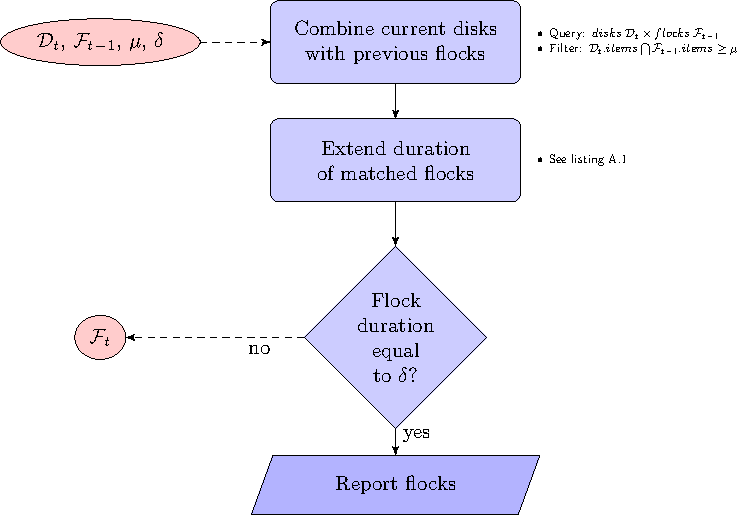
\includegraphics[width=\linewidth]{figures/FF_flowchart}
    \caption{Steps in BFE phase two. Combination, extension and reporting of flocks.}\label{fig:FF_flowchart}
\end{figure}

Similarly, Figure \ref{fig:FF_stages} illustrates the recursive process and how the set of partial flocks from previous time instants feeds into the next iteration. The example assumes a $\delta$ value of 3, meaning flocks start being reported from time instant $t_2$. Note that time instants $t_0$ and $t_1$ are considered the initial conditions. At the start of the algorithm, maximal disks are identified at $t_0$, which are immediately transformed into partial flocks with a duration of 1 and then passed on to the next time instant. At $t_1$, a new set of maximal disks $\mathcal{D}_1$ is found and joined with the partial flocks from $t_0$, denoted as $\mathcal{F}_0$. The information for each partial flock is updated accordingly, including its duration and the points it contains. From this point onward, subsequent time instants follow the exact steps outlined in Figure \ref{fig:FF_flowchart}.

\begin{figure*}
    \centering
    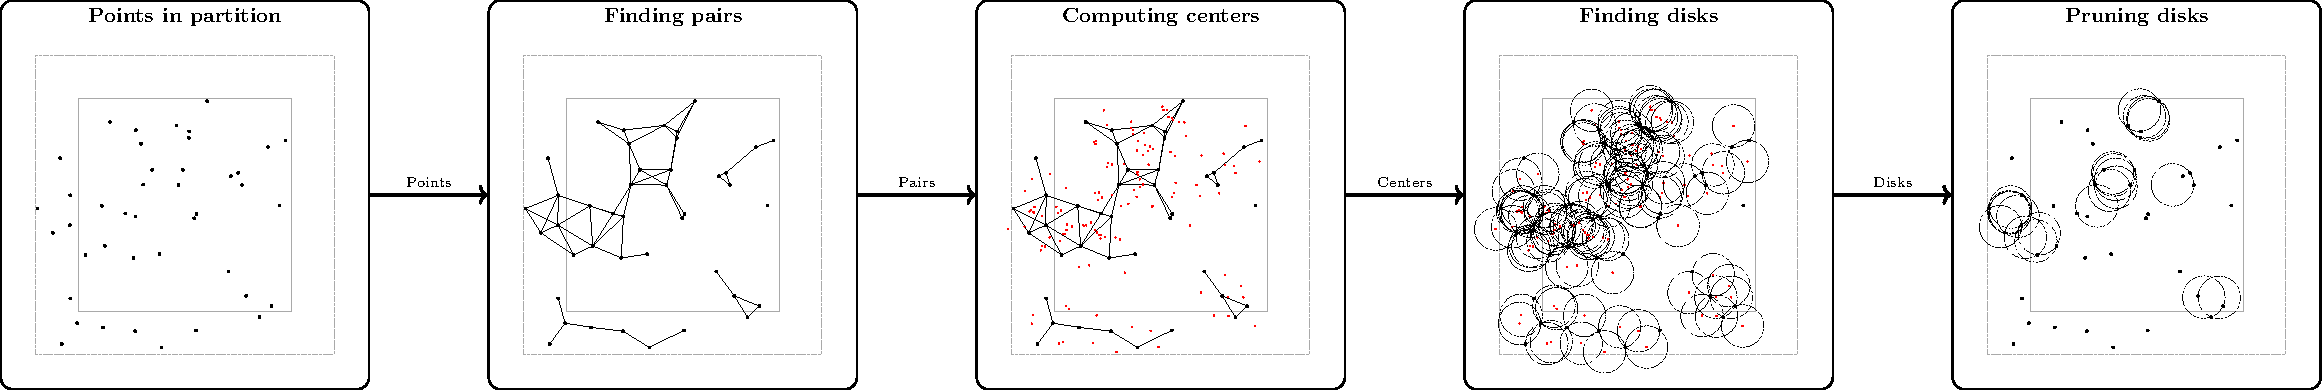
\includegraphics[width=\linewidth]{figures/MF_stages/flow}
    \caption{Example of BFE execution on a sample dataset.}\label{fig:example}
\end{figure*}

\begin{figure}[!ht]
    \centering
    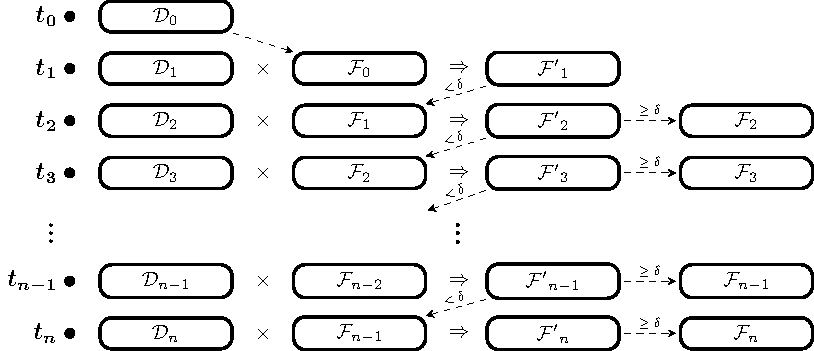
\includegraphics[width=\linewidth]{figures/FF_stages}
    \caption{BFE phase 2 example explaining the recursion of the set of flocks along time instants and the initial conditions.}\label{fig:FF_stages}
\end{figure}

\subsection{The PSI sequential algorithm}
The PSI algorithm, proposed by \cite{tanaka_improved_2016}, follows a similar process to the BFE algorithm. However, instead of using a grid structure to index points within the area, PSI employs a sweep-line approach that processes points in order of their x-coordinates. For each visited point $p$, the algorithm considers a square of side length $2\varepsilon$ centered at $p$. It only examines the points to the right of $p$ that lie within two half-squares of side length $\varepsilon$, as illustrated by the shaded regions in Figure \ref{fig:square}. 

While BFE processes points inside a grid cell of side length $\varepsilon$ along with its eight neighboring cells, PSI focuses on the points in these two half-squares. As a result, PSI more efficiently identifies the points relevant for detecting candidate pairs, centers, and disks. This indexing method has been shown to outperform BFE in most cases, with BFE offering similar or better performance only when $\varepsilon$ values are relatively small. In such cases, the number of points to consider is smaller, and PSI still requires sorting the points for the sweep-line approach. Therefore, both approaches are considered in the following sections.

\begin{figure}
    \centering
    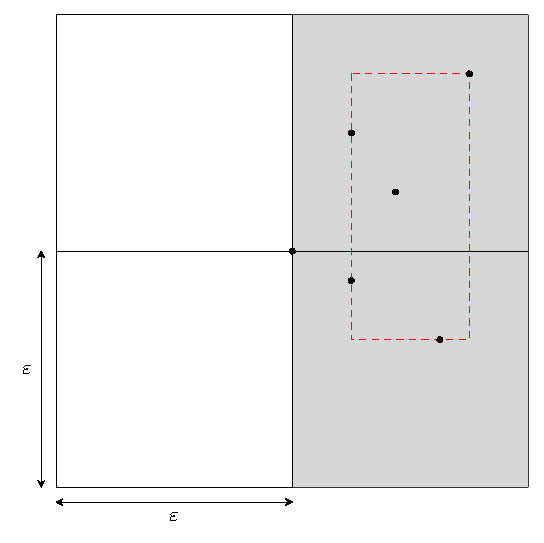
\includegraphics[width=0.5\linewidth]{figures/square.pdf}
    \caption{An example of the two half squares used in PSI algorithm.}\label{fig:square}
\end{figure}

\subsection{Bottlenecks in the sequential approach and possible solutions} \label{spatial_phase}
Since both sequential approaches follow the same steps (as shown in Figures \ref{fig:MF_flowchart} and \ref{fig:FF_flowchart}), we will focus on discussing their bottlenecks using the BFE as an example. Certain stages in the BFE process are notably impacted when handling very large datasets, which can significantly affect performance.

\subsubsection{Phase 1: Spatial finding of maximal disks.}
First, we focus on Phase 1. As illustrated in Figure \ref{fig:example}, this phase's steps are demonstrated using a sample dataset. It is important to note that the final set of maximal disks is significantly smaller than the initial number of candidate disks found. Specifically, the number of candidate centers to evaluate is $2\lvert\tau\rvert^2$, where $\tau$ represents the number of trajectories \cite{vieira_2009}. Our experiments reveal that this issue becomes more pronounced not only in very large datasets but also in those containing areas with a high density of moving entities.

To address this issue, we propose a partition-based strategy that divides the study area into smaller subareas, allowing for independent and parallel evaluation. The strategy consists of three key steps: first, the \textit{partition and replication} stage, followed by the \textit{local flock discovery} within each partition, and finally, the \textit{filtering stage}, where we consolidate and unify the results. Each of these steps is detailed below.

\begin{itemize}
    \item Partition and Replication: Figure \ref{fig:partrep} provides a brief example of the partition and replication stage. Different types of spatial indexes, such as grids, R-trees, or quadtrees, can be used to create spatial partitions of the input dataset. In the example shown in Figure \ref{fig:partrep}.b, we use a quadtree, which generates seven partitions. To ensure each partition can locally identify flocks, it must have access to all relevant data. This is achieved by replicating points that are within a distance of $\varepsilon$ from the border of each partition, an area referred to as the \textit{expansion zone}, into adjacent partitions. Figure \ref{fig:partrep}.c illustrates each partition, surrounded by a dotted line representing the expansion zone, which includes the points that need to be replicated from neighboring partitions.

    \item Local flock discovery: At this stage, each partition can be processed independently and in parallel, with partitions assigned to different processing nodes. Within each partition, we can execute the steps of Phase 1 of the BFE algorithm locally, as outlined in Figure \ref{fig:MF_flowchart}.

    \item Filtering: While partitioning and replication facilitate parallelism, they can also lead to result duplication, as different nodes may report the same maximal disk. Specifically, if a disk's center lies within a partition, it will be reported only once by the node processing that partition. However, disks with centers located in an expansion zone will be reported by all partitions that share that zone. To address this, we propose a reporting approach that effectively prevents such duplication, which we detail below.
\end{itemize}

\begin{figure}
    \centering
    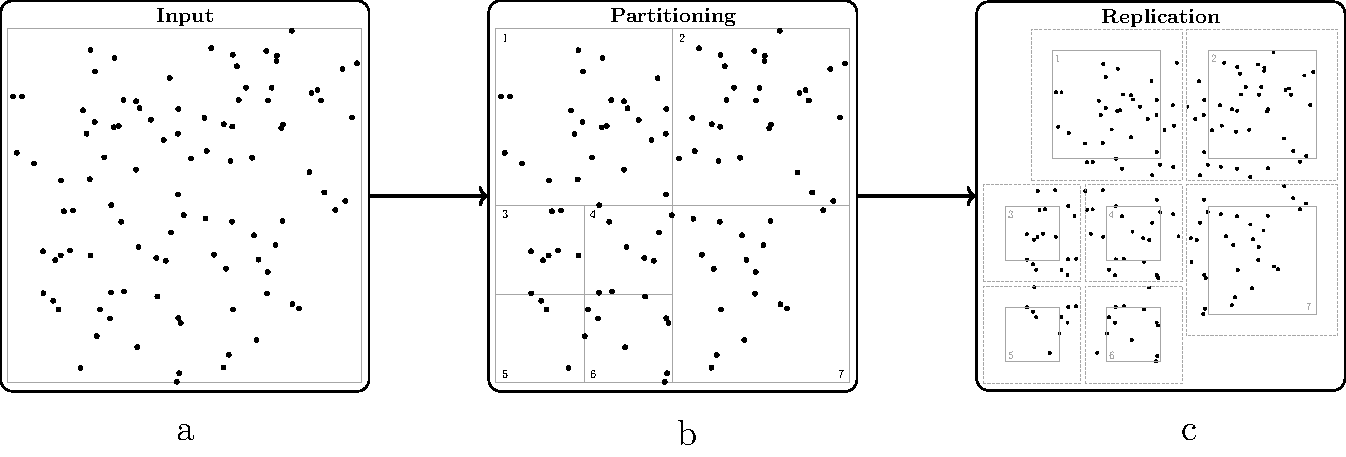
\includegraphics[width=\linewidth]{figures/MF_stages/P123}
    \caption{An example of partitioning and replication on a sample dataset.}\label{fig:partrep}
\end{figure}

Disks with centers in an expansion zone are created by points that exist in both partitions due to replication. We assert that each partition should only report disks generated within its own area and not those originating in its expansion zone. Figure \ref{fig:ensuring} illustrates the possible scenarios. Assume partitions 1 and 2 in the figure are contiguous, sharing edge AB. Consider the disks $a^\prime$ and $a^{\prime\prime}$ (each with a diameter of $\varepsilon$), which are generated by two points (shown in green) located in the expansion zone of partition 1 but inside partition 2. In this case, both $a^\prime$ and $a^{\prime\prime}$ will be reported by partition 2. Similarly, both $c^\prime$ and $c^{\prime\prime}$ will be reported by partition 1. However, $b^\prime$ will be reported by partition 1, while $b^{\prime\prime}$ will be reported by partition 2.

\begin{figure}
    \centering
    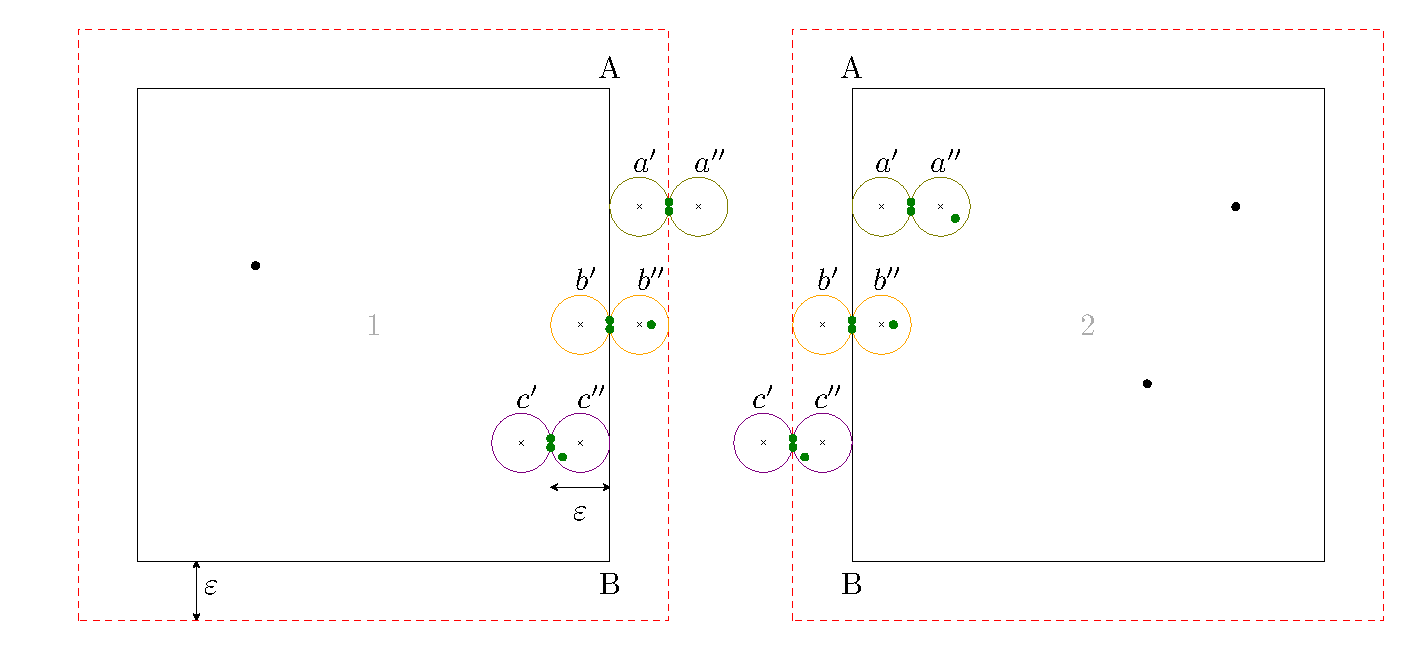
\includegraphics[width=\linewidth]{figures/merge.pdf}
    \caption{Ensuring no loss of data in safe zone and expansion area.}\label{fig:ensuring}
\end{figure}

\subsubsection{Phase 2: Temporal join}\label{sec:temporal_join}
At the end of Phase 1, we have computed a set of maximal disks for a given time instant. In Phase 2, we proceed by combining these disks over time instants to form flocks. However, since Phase 1 involved partitioning the spatial domain for parallelism, Phase 2 becomes more complex as flocks can move across spatial partitions over time. Once the maximal disks are identified for a time instant $i$, a temporal join occurs within each partition to link these disks with partial flocks from the previous time instant ($i-1$). However, we must account for partial flocks that may appear near the partition borders and potentially move into adjacent partitions (see Figure \ref{fig:simple_alternative}).

To address this issue, we introduce an additional parameter, \textit{maxdist}, which represents the maximum distance a moving object can travel between consecutive time instants. We define the \textit{safe area} of a partition as the internal region that is at least \textit{maxdist} away from the partition’s border (illustrated in grey in Figure \ref{fig:maxdist}). Any partial or full flocks discovered within a partition’s safe area can be directly reported as results. However, flocks that start or end outside the safe area must be collected for post-processing to determine if they correspond with partial flocks from neighboring partitions. These cases, where flocks cross between partitions, are referred to as \textit{crossing partial} flocks (CPFs).

\begin{figure}
    \centering
    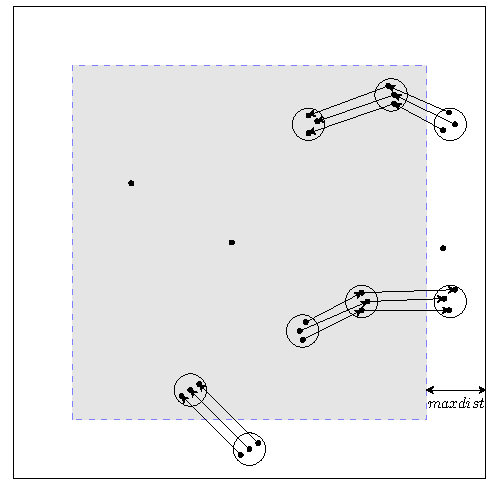
\includegraphics[width=0.7\linewidth]{figures/maxdist.pdf}
    \caption{Examples of CPFs that that start or end in the border area of a partition.}\label{fig:maxdist}
\end{figure}

\begin{figure}
    \centering
    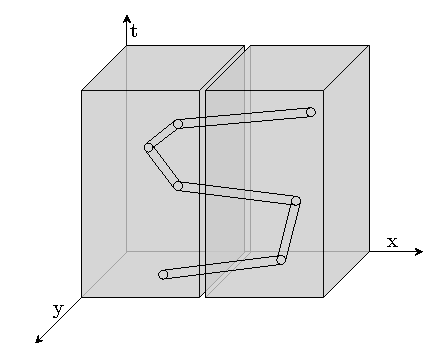
\includegraphics[width=0.8\linewidth]{figures/cubo2.pdf}
    \caption{A flock that moves in different partitions along the time.}\label{fig:simple_alternative}
\end{figure}

In the post-processing stage, we evaluate four alternatives for collecting and checking crossing partial flocks (CPFs). The simplest approach is to gather all CPFs and process them sequentially on a single node (the master node). However, due to the large number of partitions and the \textit{maxdist} parameter, the volume of CPFs requiring post-processing can become substantial, leading to a bottleneck that negatively impacts overall performance.

We also evaluate an intermediate approach where the CPFs from a given partition are sent to a middle-level node for processing, based on the quadtree structure used to create the partitions. The choice of which middle-level node to send the CPFs to is determined by a user-defined parameter called \textit{step}. A value of \textit{step=1} corresponds to sending CPFs to the immediate parent, \textit{step=2} to the grandparent, and so on, until the root is reached. For example, with \textit{step=1}, all CPFs from a partition are first sent to its parent node in the quadtree. The parent node processes its CPFs, but some flocks may still cross outside the parent's safe area.  These leftover CPFs are then passed to the next parent (since \textit{step=1}), and this process continues until all CPFs are processed, potentially reaching the root node. This approach allows for parallelism in post-processing, as moving to a parent node increases the partition's area and improves the likelihood that CPFs can be resolved at that level. In the experimental section, we test different values of the \textit{step} parameter, such as \textit{step=2}, where CPFs are sent to the grandparent at each stage.

Unlike the previous two approaches, which assign all CPFs from a given partition in the same way (partition-based), the third alternative assigns each CPF individually (CPF-based). For a given CPF $f$, we extend its most recent disk by a ring with a size of \textit{maxdist}, identifying all overlapping partitions for this extended disk—essentially determining which neighboring partitions the objects in $f$ could move to in the next time instant. For each overlapping partition, we retrieve the Least Common Ancestor (LCA) between that partition and $f$'s original partition. CPF $f$ is then sent to the node(s) corresponding to these LCAs. The benefit of this approach is that the LCA can efficiently complete the processing for $f$, as it exploits proximity using \textit{mindist}. However, the downside is the increased copying overhead, as $f$ may need to be sent to multiple nodes.

A limitation of the previous alternatives is that each spatial partition is processed by a single node, which incrementally evaluates all time instances for that partition. The fourth alternative introduces fixed divisions in the temporal domain, based on a user-defined parameter (number of divisions), as illustrated in Figure \ref{fig:cube_alternative}. In this approach, the spatio-temporal space is divided into temporal 'cubes,' each of which can be processed by different nodes. For simplicity, we assume that each division spans the same length of time. However, an additional validation step is required to ensure continuity of flocks across temporal divisions.

\begin{figure}
    \centering
    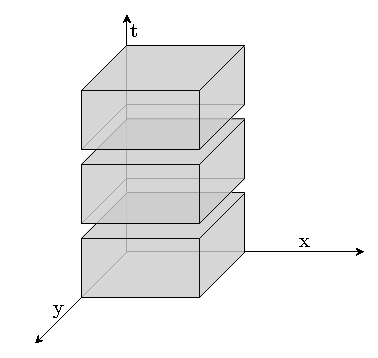
\includegraphics[width=0.8\linewidth]{figures/cubo.pdf}
    \caption{An alternative division on the time dimension to partition the data into cubes.}\label{fig:cube_alternative}
\end{figure}
